\documentclass[11pt,a4paper]{article}
\usepackage[utf8]{inputenc}
\usepackage[margin=2.5cm]{geometry}
\usepackage{amsmath}
\usepackage{xcolor}
\usepackage{booktabs}
\usepackage{tabularx}
\usepackage{array}
\usepackage{listings}
\usepackage{tikz}
\usetikzlibrary{arrows.meta,positioning,shapes.multipart}
\usepackage{fancyhdr}
\usepackage{enumitem}
\usepackage[hidelinks]{hyperref}

\renewcommand{\tablename}{Tabla}
\renewcommand{\figurename}{Figura}
\renewcommand{\contentsname}{Contenido}
\definecolor{azul}{RGB}{31,78,121}
\definecolor{gris}{RGB}{245,245,245}
\definecolor{verde}{RGB}{0,110,60}
\definecolor{rojo}{RGB}{160,30,30}

\lstset{
  language=C, basicstyle=\ttfamily\footnotesize, backgroundcolor=\color{gris},
  keywordstyle=\color{azul}\bfseries, commentstyle=\color{verde}\itshape,
  stringstyle=\color{rojo}, frame=single, rulecolor=\color{azul!40},
  breaklines=true, columns=fullflexible, showstringspaces=false,
  xleftmargin=0.5em, xrightmargin=0.5em, aboveskip=0.8em, belowskip=0.8em
}

\newcommand{\fn}[1]{\texttt{\detokenize{#1}}}
\newcommand{\pendiente}[1]{\textcolor{rojo}{[#1]}}

%integrantes
\newcommand{\integranteA}{Israel Becerra}
\newcommand{\integranteB}{Benjamin Borquez}

\setlist{itemsep=2pt,topsep=4pt}
\pagestyle{fancy}
\fancyhf{}
\fancyhead[L]{\small Proyecto 2: RPG de texto}
\fancyhead[R]{\small Estructura de Datos}
\fancyfoot[C]{\thepage}
\renewcommand{\headrulewidth}{0.4pt}

\setlength{\emergencystretch}{4em}
\begin{document}

% ================= PORTADA =================
\begin{titlepage}
\centering
\vspace*{2cm}
{\Large\color{azul} Estructura de Datos\par}
\vspace{1.2cm}
{\Huge\bfseries\color{azul} Proyecto 2: Juego RPG\par}
\vspace{0.4cm}
{\large Listas enlazadas, pilas y colas en C\par}
\vspace{2cm}
\begin{tabular}{rl}
\textbf{Docente:} & Jacqueline Aldridge \\
\textbf{Integrantes:} & \integranteA \\
 & \integranteB \\
\textbf{Fecha de entrega:} & 30 de octubre de 2026 \\
\textbf{Lenguaje:} & C \\
\end{tabular}
\vfill
\end{titlepage}

\tableofcontents
\newpage

% ================= 1. INTRODUCCION =================
\section{Introduccion}
Este proyecto implementa una version simplificada de un juego de rol por terminal.
El personaje explora una zona, encuentra objetos, administra su inventario,
enfrenta enemigos y puede guardar y cargar su partida. Todo el sistema se
construyo con tres estructuras implementadas por el grupo, sin bibliotecas que
las resuelvan:

\begin{itemize}
  \item una \textbf{lista enlazada} para el inventario,
  \item una \textbf{pila} para el historial de acciones y el deshacer,
  \item una \textbf{cola} para el orden de combate contra varios enemigos.
\end{itemize}

Cada estructura participa en funcionalidades reales del juego: no se crearon
solo para mostrar sus elementos. En este informe se justifica la eleccion de cada una,
se explican sus operaciones, como se respeta el tipo de dato abstracto (TDA) y
como se manejan los casos limite (estructura vacia, un solo elemento, memoria
insuficiente y eliminacion).

% ================= OBJETIVOS =================
\section{Objetivos}

\subsection{Objetivo general}
Diseñar e implementar en lenguaje C un juego de rol por terminal, utilizando listas
enlazadas, pilas y colas implementadas por el grupo, de modo que cada estructura
participe en las funcionalidades del juego y se manejen correctamente los casos
limite.

\subsection{Objetivos especificos}
\begin{enumerate}
  \item Implementar el inventario del personaje como una lista enlazada que permita agregar,
        listar, buscar por nombre o ID, usar y eliminar objetos.
  \item Implementar el historial de acciones como una pila, mostrandolo de la accion mas reciente
        a la mas antigua y permitiendo deshacer el descarte de un objeto.
  \item Implementar una cola para enfrentar a varios enemigos en su orden de aparicion.
  \item Desarrollar la exploracion por pasos con eventos al azar (nada, objeto o enemigos) y un combate
        por turnos que use el inventario.
  \item Permitir guardar y cargar la partida mediante archivos, validando que los datos sean correctos.
  \item Manejar los casos de estructura vacia, un solo elemento, memoria insuficiente y eliminacion,
        liberando toda la memoria reservada para evitar fugas.
  \item Validar las entradas del usuario y mostrar mensajes claros ante operaciones invalidas.
  \item Verificar el funcionamiento mediante pruebas de casos limite y documentar las decisiones de diseño.
\end{enumerate}

% ================= 2. DISENO GENERAL =================
\section{Diseño general}
El codigo esta dividido en modulos pequeños, cada uno con su archivo \fn{.h}
(contrato) y su archivo \fn{.c} (implementacion).

\begin{table}[h]
\centering
\small
\begin{tabularx}{\textwidth}{l l X}
\toprule
\textbf{Modulo} & \textbf{Estructura} & \textbf{Funcion en el juego} \\
\midrule
\fn{objeto} & struct & Datos de un objeto: ID, nombre, tipo, valor. \\
\fn{personaje} & struct & Nombre, vida, ataque y defensa; recibir daño y curar. \\
\fn{inventario} & \textbf{lista enlazada} & Guardar, buscar, usar y eliminar objetos. \\
\fn{historial} & \textbf{pila} & Registrar acciones y mostrarlas de la mas reciente a la mas antigua. \\
\fn{acciones} & usa pila y lista & Descartar objetos y deshacer el descarte. \\
\fn{enemigo} & struct & Datos del enemigo: vida, daño, turnos dormido. \\
\fn{cola_combate} & \textbf{cola} & Orden en que se enfrentan los enemigos. \\
\fn{combate} & usa cola, lista y pila & Bucle de combate por turnos. \\
\fn{aventura} & usa cola, lista y pila & Exploracion por pasos y eventos al azar. \\
\fn{guardado} & archivos & Guardar y cargar la partida. \\
\fn{entrada} & --- & Lectura validada de numeros, texto y respuestas s/n. \\
\fn{menu}, \fn{main} & --- & Menu por terminal y arranque del programa. \\
\bottomrule
\end{tabularx}
\caption{Modulos del proyecto.}
\end{table}

\begin{figure}[h]
\centering
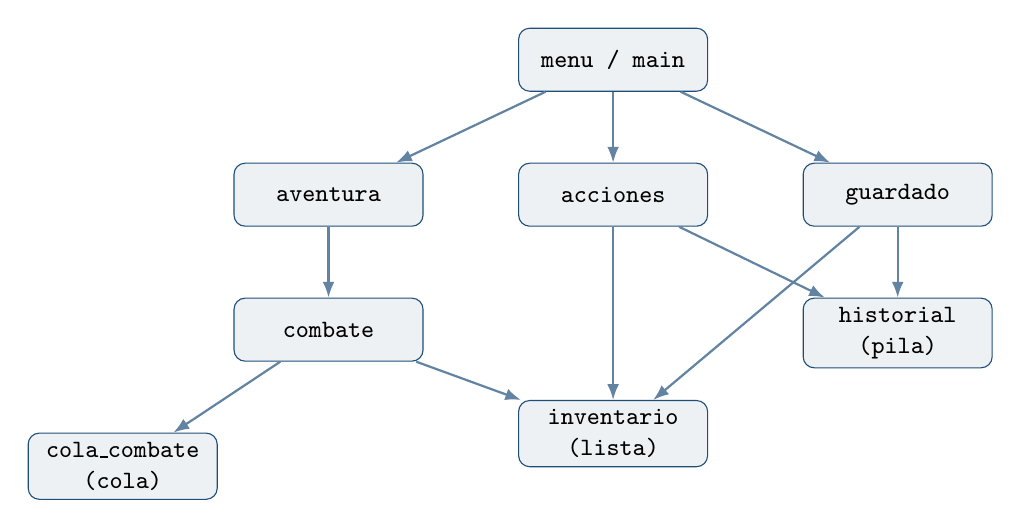
\begin{tikzpicture}[
  caja/.style={draw=azul,fill=azul!8,rounded corners,minimum width=2.4cm,minimum height=0.8cm,font=\small\ttfamily,align=center},
  flecha/.style={-{Latex[length=2mm]},thick,azul!70}]
  \node[caja] (menu) {menu / main};
  \node[caja,below left=0.9cm and 1.2cm of menu] (aventura) {aventura};
  \node[caja,below=0.9cm of menu] (acciones) {acciones};
  \node[caja,below right=0.9cm and 1.2cm of menu] (guardado) {guardado};
  \node[caja,below=0.9cm of aventura] (combate) {combate};
  \node[caja,below=2.2cm of acciones] (inventario) {inventario\\(lista)};
  \node[caja,below=0.9cm of guardado] (historial) {historial\\(pila)};
  \node[caja,below left=0.9cm and 0.2cm of combate] (cola) {cola\_combate\\(cola)};
  \draw[flecha] (menu)--(aventura);
  \draw[flecha] (menu)--(acciones);
  \draw[flecha] (menu)--(guardado);
  \draw[flecha] (aventura)--(combate);
  \draw[flecha] (combate)--(cola);
  \draw[flecha] (combate)--(inventario);
  \draw[flecha] (acciones)--(inventario);
  \draw[flecha] (acciones)--(historial);
  \draw[flecha] (guardado)--(historial);
  \draw[flecha] (guardado)--(inventario);
\end{tikzpicture}
\caption{Dependencias principales entre modulos (una flecha significa ``usa'').}
\end{figure}

\paragraph{Reglas de diseño.} Las funciones de cada estructura reciben el
puntero a la estructura y devuelven un codigo (0 si todo salio bien, un valor
negativo si hubo error), lo que permite que quien llama decida que mensaje
mostrar. Los mensajes al usuario se escriben en el menu y en los modulos de
juego, no dentro de las estructuras (salvo los de listado).

% ================= 3. ESTRUCTURAS =================
\section{Estructuras de datos}

\subsection{Inventario: lista enlazada simple}

\paragraph{Definicion.}
Cada nodo guarda un \fn{Objeto} y un puntero al siguiente. El inventario guarda la
\fn{cabeza} y la \fn{cantidad}.

\begin{lstlisting}
typedef struct NodoInventario {
    Objeto objeto;
    struct NodoInventario *siguiente;
} NodoInventario;

typedef struct { NodoInventario *cabeza; int cantidad; } Inventario;
\end{lstlisting}

\begin{figure}[h]
\centering
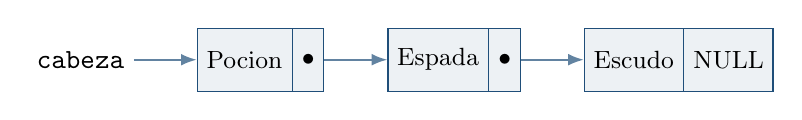
\begin{tikzpicture}[
  nodo/.style={rectangle split,rectangle split parts=2,rectangle split horizontal,draw=azul,fill=azul!8,minimum height=0.8cm,font=\small},
  flecha/.style={-{Latex[length=2mm]},thick,azul!70}]
  \node (c) {\fn{cabeza}};
  \node[nodo,right=0.8cm of c] (a) {Pocion\nodepart{two}$\bullet$};
  \node[nodo,right=0.8cm of a] (b) {Espada\nodepart{two}$\bullet$};
  \node[nodo,right=0.8cm of b] (d) {Escudo\nodepart{two}NULL};
  \draw[flecha] (c)--(a.west);
  \draw[flecha] (a.two east)--(b.west);
  \draw[flecha] (b.two east)--(d.west);
\end{tikzpicture}
\caption{Inventario como lista enlazada.}
\end{figure}

\paragraph{Por que una lista enlazada y no otra estructura.}
El inventario necesita buscar por nombre o ID y eliminar un objeto de
\emph{cualquier} posicion (por ejemplo, descartar el segundo objeto o gastar una
pocion). Una pila solo permite sacar el tope y una cola solo el frente, por lo
que no sirven. Un arreglo fijo limita la cantidad de objetos y obliga a
desplazar elementos al eliminar; la lista crece segun se necesita y eliminar
solo reasigna un puntero.

\paragraph{Operaciones implementadas.}
\begin{table}[h]
\centering
\small
\begin{tabularx}{\textwidth}{l X c}
\toprule
\textbf{Operacion} & \textbf{Descripcion} & \textbf{Costo} \\
\midrule
\fn{inventario_iniciar} & Deja la lista vacia (\fn{cabeza = NULL}). & $O(1)$ \\
\fn{inventario_agregar} & Reserva un nodo y lo agrega al final. & $O(n)$ \\
\fn{inventario_listar} & Recorre e imprime todos los objetos. & $O(n)$ \\
\fn{inventario_buscar_por_nombre} & Devuelve el nodo con ese nombre o \fn{NULL}. & $O(n)$ \\
\fn{inventario_buscar_por_id} & Igual, comparando el ID. & $O(n)$ \\
\fn{inventario_eliminar_por_id} & Quita el nodo y entrega una copia del objeto. & $O(n)$ \\
\fn{inventario_usar_objeto} & Aplica el efecto segun el tipo del objeto. & $O(n)$ \\
\fn{inventario_liberar} & Libera todos los nodos. & $O(n)$ \\
\bottomrule
\end{tabularx}
\caption{Operaciones del inventario.}
\end{table}

Agregar al final cuesta $O(n)$ porque se recorre la lista hasta el ultimo nodo;
se acepto porque los inventarios del juego son pequeños y asi se conserva el orden
en que se recogen los objetos. Si se quisiera $O(1)$ bastaria agregar un puntero al
final, como se hace en la cola.

\paragraph{Eliminacion.}
\fn{inventario_eliminar_por_id} usa dos punteros, \fn{actual} y \fn{anterior}. Con
ellos distingue los casos: lista vacia, eliminar la cabeza (que incluye el caso de un
solo elemento) y eliminar un nodo intermedio o el ultimo.

\begin{lstlisting}
if (anterior == NULL) {         /* es la cabeza (o unico elemento) */
    inv->cabeza = actual->siguiente;
} else {                        /* nodo intermedio o ultimo */
    anterior->siguiente = actual->siguiente;
}
if (eliminado != NULL) { *eliminado = actual->objeto; }  /* copia para deshacer */
free(actual);
inv->cantidad--;
\end{lstlisting}

\paragraph{Uso de objetos.}
\fn{inventario_usar_objeto} copia el objeto antes de actuar, porque si es una
pocion el nodo se libera. Una \textbf{pocion} cura (\fn{personaje_curar}) y se elimina
del inventario; un \textbf{arma} suma su valor al ataque; una \textbf{armadura} suma su
valor a la defensa; las armas y armaduras permanecen en el inventario.

\subsection{Historial: pila}

\paragraph{Definicion.}
Cada nodo guarda una \fn{Accion} (tipo, descripcion y una copia del objeto
descartado) y apunta al nodo de abajo. La pila guarda solo el \fn{top}.

\begin{lstlisting}
typedef struct NodoHistorial {
    Accion accion;
    struct NodoHistorial *siguiente;   /* el que esta debajo */
} NodoHistorial;

typedef struct { NodoHistorial *top; int cantidad; } Historial;
\end{lstlisting}

\begin{figure}[h]
\centering
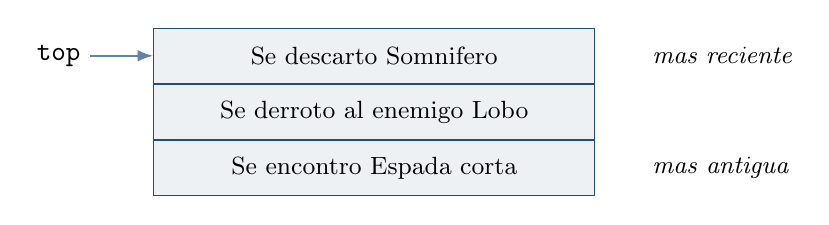
\begin{tikzpicture}[
  celda/.style={draw=azul,fill=azul!8,minimum width=5.6cm,minimum height=0.7cm,font=\small},
  flecha/.style={-{Latex[length=2mm]},thick,azul!70}]
  \node[celda] (a) {Se descarto Somnifero};
  \node[celda,below=0pt of a] (b) {Se derroto al enemigo Lobo};
  \node[celda,below=0pt of b] (c) {Se encontro Espada corta};
  \node[left=0.8cm of a] (t) {\fn{top}};
  \draw[flecha] (t)--(a);
  \node[right=0.6cm of a,font=\small\itshape] {mas reciente};
  \node[right=0.6cm of c,font=\small\itshape] {mas antigua};
\end{tikzpicture}
\caption{Historial como pila (LIFO).}
\end{figure}

\paragraph{Por que una pila.}
El enunciado pide mostrar las acciones de la mas reciente a la mas antigua y
deshacer \emph{solo la ultima} accion. Ambos requisitos son LIFO: lo ultimo que
entra es lo primero que se ve y lo primero que se puede deshacer. No hace falta acceder
a posiciones intermedias.

\paragraph{Operaciones y respeto del TDA.}
\begin{table}[h]
\centering
\small
\begin{tabularx}{\textwidth}{l X c}
\toprule
\textbf{Operacion} & \textbf{Descripcion} & \textbf{Costo} \\
\midrule
\fn{historial_push} & Agrega una accion arriba: el nuevo nodo apunta al antiguo tope. & $O(1)$ \\
\fn{historial_pop} & Saca la accion del tope y libera su nodo. & $O(1)$ \\
\fn{historial_peek} & Copia la accion del tope sin sacarla. & $O(1)$ \\
\fn{historial_esta_vacio} & Indica si no hay acciones. & $O(1)$ \\
\fn{historial_mostrar} & Imprime desde el tope hacia abajo, sin modificar. & $O(n)$ \\
\fn{historial_liberar} & Libera todos los nodos. & $O(n)$ \\
\bottomrule
\end{tabularx}
\caption{Operaciones de la pila.}
\end{table}

Las operaciones que modifican la pila (\fn{push} y \fn{pop}) y la que consulta
(\fn{peek}) solo tocan el \emph{tope}, sin recorrer nada. El unico recorrido en el
propio modulo es \fn{historial_mostrar}, que es de solo lectura y existe porque el
enunciado pide ver todo el historial. El modulo \fn{guardado} tambien recorre los
nodos para escribir la pila en el archivo, y lo hace sin modificarlos. En la logica
del juego (combate, aventura y acciones) la pila se usa solo mediante \fn{push},
\fn{pop} y \fn{peek}.

\paragraph{Deshacer.}
El enunciado permite deshacer solo si la ultima accion fue descartar un objeto.
\fn{deshacer_ultima_accion} hace \fn{peek}; si el tipo no es
\fn{ACCION_DESCARTAR_OBJETO}, informa que no se puede deshacer y la pila queda
intacta. Si lo es, devuelve el objeto al inventario y recien entonces hace \fn{pop}.

\begin{lstlisting}
if (historial_peek(h, &accion) != 0)            return ACCION_ERR_VACIO;
if (accion.tipo != ACCION_DESCARTAR_OBJETO)     return ACCION_ERR_NO_DESHACER;
if (inventario_buscar_por_id(inv, accion.objeto_descartado.id) != NULL)
                                                return ACCION_ERR_ID_REPETIDO;
/* Primero se devuelve el objeto: si falla, el historial queda intacto. */
if (inventario_agregar(inv, accion.objeto_descartado) != 0)
                                                return ACCION_ERR_MEMORIA;
historial_pop(h, &accion);
return ACCION_OK;
\end{lstlisting}

Este orden (primero agregar, despues \fn{pop}) evita perder el objeto si no hay memoria.

\subsection{Cola de combate: cola enlazada}

\paragraph{Definicion.}
La cola guarda dos punteros: \fn{frente} (por donde sale el siguiente enemigo) y
\fn{final} (por donde entra el nuevo), mas la \fn{cantidad}.

\begin{lstlisting}
typedef struct NodoCola {
    Enemigo enemigo;
    struct NodoCola *siguiente;
} NodoCola;

typedef struct { NodoCola *frente; NodoCola *final; int cantidad; } ColaCombate;
\end{lstlisting}

\begin{figure}[h]
\centering
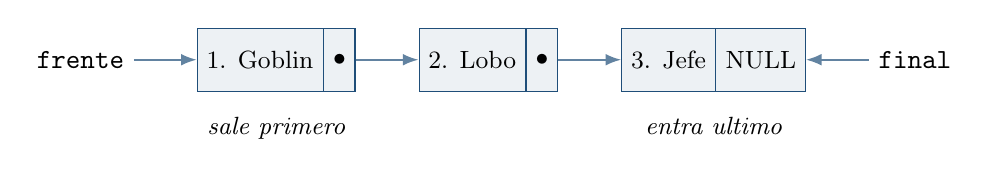
\begin{tikzpicture}[
  nodo/.style={rectangle split,rectangle split parts=2,rectangle split horizontal,draw=azul,fill=azul!8,minimum height=0.8cm,font=\small},
  flecha/.style={-{Latex[length=2mm]},thick,azul!70}]
  \node (f) {\fn{frente}};
  \node[nodo,right=0.8cm of f] (a) {1. Goblin\nodepart{two}$\bullet$};
  \node[nodo,right=0.8cm of a] (b) {2. Lobo\nodepart{two}$\bullet$};
  \node[nodo,right=0.8cm of b] (c) {3. Jefe\nodepart{two}NULL};
  \node[right=0.8cm of c] (fin) {\fn{final}};
  \draw[flecha] (f)--(a.west);
  \draw[flecha] (a.two east)--(b.west);
  \draw[flecha] (b.two east)--(c.west);
  \draw[flecha] (fin)--(c.east);
  \node[below=0.2cm of a,font=\small\itshape] {sale primero};
  \node[below=0.2cm of c,font=\small\itshape] {entra ultimo};
\end{tikzpicture}
\caption{Cola de combate (FIFO).}
\end{figure}

\paragraph{Por que una cola.}
Cada enemigo tiene un numero de aparicion y deben enfrentarse en ese orden:
primero el 1, luego el 2 y asi. Es FIFO: el primero en entrar es el primero en
salir. Una pila los enfrentaria al reves, y una lista permitiria sacar enemigos
saltandose el orden, lo que el juego no debe permitir. Se usa un puntero \fn{final}
para que encolar sea $O(1)$ sin recorrer la cola.

\paragraph{Operaciones y respeto del TDA.}
\begin{table}[h]
\centering
\small
\begin{tabularx}{\textwidth}{l X c}
\toprule
\textbf{Operacion} & \textbf{Descripcion} & \textbf{Costo} \\
\midrule
\fn{cola_iniciar} & Deja \fn{frente}, \fn{final} y \fn{cantidad} en vacio. & $O(1)$ \\
\fn{cola_encolar} & Agrega un enemigo al final. & $O(1)$ \\
\fn{cola_desencolar} & Saca el enemigo del frente. & $O(1)$ \\
\fn{cola_frente} & Copia el enemigo del frente sin sacarlo. & $O(1)$ \\
\fn{cola_esta_vacia} & Indica si no hay enemigos. & $O(1)$ \\
\fn{cola_liberar} & Desencola hasta vaciar la cola. & $O(n)$ \\
\bottomrule
\end{tabularx}
\caption{Operaciones de la cola.}
\end{table}

El modulo de combate solo usa \fn{cola_desencolar}, \fn{cola_esta_vacia} y el
contador \fn{cantidad}: nunca recorre ni modifica los nodos. Quien arma el grupo
(\fn{aventura}) solo usa \fn{cola_iniciar}, \fn{cola_encolar} y \fn{cola_liberar}, creando los enemigos con numeros de
aparicion 1, 2, 3, \ldots{} en ese orden.

\begin{lstlisting}
int cola_desencolar(ColaCombate *c, Enemigo *e) {
    if (cola_esta_vacia(c)) return -1;
    NodoCola *nodo = c->frente;
    c->frente = nodo->siguiente;
    if (c->frente == NULL) {            /* era el unico: final tambien en NULL */
        c->final = NULL;
    }
    if (e != NULL) *e = nodo->enemigo;
    free(nodo);
    c->cantidad--;
    return 0;
}
\end{lstlisting}

\subsection{Otras estructuras}
\fn{Objeto}, \fn{Personaje}, \fn{Enemigo} y \fn{Accion} son \fn{struct} simples sin
punteros. El \fn{Enemigo} incluye el campo \fn{turnos\_dormido}, que permite el
efecto del somnifero (el enemigo pierde su ataque durante N turnos).

% ================= 4. ALGORITMOS =================
\section{Algoritmos y funcionalidades}

\subsection{Exploracion}
El jugador elige una zona (Bosque Sombrio, Cueva Humeda o Ruinas Antiguas; a mayor
dificultad, enemigos mas fuertes). La exploracion avanza paso a paso y \textbf{cada 3 pasos}
se genera un evento al azar con \fn{rand() \% 3}: nada, un objeto en el suelo o un
grupo de enemigos. Tras un objeto o un combate se pregunta si se sigue explorando.

\begin{itemize}
  \item \textbf{Objeto:} se elige al azar de una tabla, recibe un ID entre 100 y 999 que no exista en el inventario,
        se registra en el historial (``Se encontro X'') y el jugador decide si lo recoge.
  \item \textbf{Enemigos:} se crean 2 o 3 enemigos de la zona, se encolan con su numero de aparicion y se llama
        al combate. Al terminar se libera la cola, incluidos los enemigos que no se enfrentaron.
\end{itemize}

\subsection{Combate}
Los enemigos salen de la cola en orden. En cada turno el jugador puede:

\begin{enumerate}
  \item \textbf{Atacar:} el enemigo pierde vida igual al ataque del personaje. Gasta turno.
  \item \textbf{Ver inventario:} lista los objetos. No gasta turno.
  \item \textbf{Usar objeto:} por ID. Gasta turno. Un objeto de tipo \emph{otro} (somnifero) duerme al enemigo
        actual N turnos; una pocion cura; un arma o armadura se equipa.
\end{enumerate}

Si el turno se gasto y el enemigo sigue vivo, el enemigo responde: si esta
dormido pierde el turno y se descuenta uno; si no, ataca. El daño que recibe
el personaje es $\max(0,\ \text{daño del enemigo} - \text{defensa})$ y la vida nunca baja de 0.
Cuando un enemigo cae se registra en el historial (``Se derroto al enemigo X'') y se pasa al siguiente de la cola.
El combate termina con victoria (cola vacia), con la muerte del personaje o si se
acaba la entrada. Un personaje sin vida no puede explorar.

\subsection{Descartar objetos y deshacer}
El jugador puede eliminar un objeto por ID o por nombre. \fn{descartar_objeto_por_id}
lo saca del inventario, guarda una copia en la accion del historial y hace \fn{push}.
Si el \fn{push} falla por falta de memoria, el objeto se devuelve al inventario y no se pierde nada.

\subsection{Guardado y carga}
La partida se guarda en un archivo de texto (\fn{saves/partida.txt}) con una linea por registro:

\begin{lstlisting}[language={}]
RPG_SAVE_2
P Aria 28 30 8 2            personaje: nombre vida vida_max ataque defensa
I 2                         cantidad de objetos, y luego una linea O por objeto
O 1 Pocion_menor 2 20
O 310 Espada_corta 0 5
H 2                         cantidad de acciones (de la mas antigua a la mas reciente)
A 0 Se_encontro_Espada_corta 0 \e 0 0
A 3 Se_descarto_Somnifero 2 Somnifero 3 2
\end{lstlisting}

\begin{itemize}
  \item Los textos se codifican como una sola palabra: el espacio pasa a \fn{\_}, el \fn{\_} real a \fn{\textbackslash\_} y el texto vacio a \fn{\textbackslash e}.
        Asi los nombres con espacios o guiones bajos se cargan igual que se guardaron.
  \item El historial se escribe de la mas antigua a la mas reciente, de modo que al cargar, haciendo \fn{push} en ese orden, el tope queda en la accion mas reciente.
  \item Al cargar, todo se lee en estructuras temporales y solo si el archivo es valido se reemplaza la partida actual. Un archivo inexistente o dañado devuelve error y no se pierde la partida en curso.
\end{itemize}

\subsection{Entrada de datos}
El modulo \fn{entrada} lee siempre una linea completa y valida: rechaza letras, texto
mezclado con numeros (``12abc''), numeros fuera de rango y respuestas distintas de
\fn{s}/\fn{n}, y descarta lo que sobre de una linea muy larga. Todas las funciones
que piden datos usan este modulo.

% ================= 5. CASOS LIMITE =================
\section{Manejo de casos limite}

\begin{table}[h]
\centering
\small
\begin{tabularx}{\textwidth}{l X}
\toprule
\textbf{Caso} & \textbf{Como se maneja} \\
\midrule
\multicolumn{2}{l}{\textit{Estructura vacia}} \\
Inventario & \fn{listar} muestra ``El inventario esta vacio''; \fn{eliminar} y \fn{buscar} devuelven error o \fn{NULL}. \\
Historial & \fn{pop} y \fn{peek} devuelven $-1$; \fn{mostrar} avisa que esta vacio; deshacer informa ``No hay acciones para deshacer''. \\
Cola & \fn{desencolar} y \fn{frente} devuelven $-1$; el combate avisa ``No hay enemigos''. \\
\midrule
\multicolumn{2}{l}{\textit{Un solo elemento}} \\
Lista & Eliminar la cabeza cuando es el unico deja \fn{cabeza = NULL} y \fn{cantidad = 0}. \\
Pila & \fn{pop} del unico nodo deja \fn{top = NULL} sin caso especial. \\
Cola & Al sacar el unico, \fn{frente} queda en \fn{NULL} y \fn{final} tambien; sin esto el siguiente \fn{encolar} escribiria en memoria liberada. \\
\midrule
\multicolumn{2}{l}{\textit{Memoria insuficiente}} \\
Todas las estructuras & Se revisa si \fn{malloc} devuelve \fn{NULL} antes de usar el nodo; la funcion devuelve $-1$ y la estructura queda sin cambios. \\
Descartar & Si falla el \fn{push}, el objeto vuelve al inventario. \\
Deshacer & Primero se agrega al inventario y solo despues se hace \fn{pop}. \\
Aventura & Si falla al crear enemigos, se libera la cola parcial y se interrumpe la exploracion con un mensaje. \\
Cargar & Se carga en estructuras temporales y se liberan si algo falla. \\
\midrule
\multicolumn{2}{l}{\textit{Eliminacion y liberacion}} \\
Eliminacion & Cabeza, nodo intermedio, ultimo y ID inexistente (devuelve $-1$). \\
Liberacion & \fn{inventario_liberar}, \fn{historial_liberar} y \fn{cola_liberar} recorren la estructura guardando el siguiente antes de hacer \fn{free}. Al salir del programa se liberan inventario e historial. \\
\bottomrule
\end{tabularx}
\caption{Casos limite por estructura.}
\end{table}

% ================= 6. EJEMPLOS =================
\section{Ejemplos de ejecucion}

\subsection{Exploracion, objeto y combate}
\begin{lstlisting}[language={}]
Zonas disponibles:
1. Bosque Sombrio (dificultad baja)
2. Cueva Humeda (dificultad media)
3. Ruinas Antiguas (dificultad alta)
0. Volver
> 1
Entras a Bosque Sombrio...
Caminas entre los arboles.
No encuentras nada.
Sigues por el sendero.
No encuentras nada.
Cruzas un pequeno arroyo.
Encuentras un objeto en el suelo!
 [310] Espada corta (arma, +5 ataque)
Deseas recogerlo? (s/n) > s
Espada corta agregado al inventario.
\end{lstlisting}

\begin{lstlisting}[language={}]
Un grupo de enemigos te bloquea el paso!
Enemigos:
 1. Goblin (15 PV)
 2. Lobo (20 PV)

===== COMBATE =====
Aria: 30/30 PV | Ataque 8 | Defensa 2
Enemigo actual: Goblin (15/15 PV)
Enemigos en espera: 1
1. Atacar
2. Ver inventario
3. Usar objeto
> 1
Atacas a Goblin: 8 de dano. Goblin: 7/15 PV.
Goblin te ataca: recibes 2 de dano. Aria: 28/30 PV.
...
Atacas a Goblin: 8 de dano. Goblin: 0/15 PV.
Derrotaste a Goblin!
\end{lstlisting}

El Goblin (numero 1) se enfrenta antes que el Lobo (numero 2) porque la cola respeta el orden de aparicion.

\subsection{Descartar y deshacer}
\begin{lstlisting}[language={}]
Nombre > Somnifero
Se descarto Somnifero. Puedes deshacerlo desde el historial.

===== HISTORIAL =====
- Se descarto Somnifero
- Se encontro Espada corta

> 2    (Deshacer ultima accion)
Se deshizo el descarte: el objeto volvio al inventario.
\end{lstlisting}

% ================= 7. PRUEBAS =================
\section{Pruebas realizadas}

\subsection{Pruebas de casos limite}
Las pruebas se hicieron de forma manual, ejecutando el juego y usando sus menus, con atencion especial a
los casos limite que pide el enunciado: estructura vacia, un solo elemento y eliminacion. Se probaron las
tres estructuras (lista, pila y cola), el descartar y deshacer, el guardado y la carga de partida, y las
entradas invalidas del usuario. Para cada caso se indica el resultado esperado y si el programa se
comporto como se esperaba (Tabla~\ref{tab:pruebas}). Los casos de memoria insuficiente se revisaron en el
codigo: cada \fn{malloc} verifica si devolvio \fn{NULL} antes de usar el nodo y la funcion retorna $-1$ sin
modificar la estructura.

\begin{table}[h]
\centering
\small
\begin{tabularx}{\textwidth}{l X c}
\toprule
\textbf{Prueba} & \textbf{Resultado esperado} & \textbf{Resultado} \\
\midrule
Desencolar en cola vacia & Devuelve $-1$, sin error & Correcto \\
Cola con un elemento, desencolar & \fn{frente} y \fn{final} en \fn{NULL} & Correcto \\
Encolar 1, 2, 3 y desencolar & Salen en orden 1, 2, 3 (FIFO) & Correcto \\
\fn{pop} y \fn{peek} en pila vacia & Devuelven $-1$ & Correcto \\
\fn{push} A, B y \fn{pop} & Sale B y luego A (LIFO) & Correcto \\
\fn{peek} con elementos & No saca nada; la cantidad no cambia & Correcto \\
Eliminar cabeza, medio, ultimo y unico & La lista queda coherente & Correcto \\
Eliminar ID inexistente & Devuelve $-1$ & Correcto \\
Deshacer tras descartar & El objeto vuelve y se saca de la pila & Correcto \\
Deshacer tras otra accion & Mensaje ``no se puede deshacer'' & Correcto \\
Guardar y cargar & Personaje, inventario e historial iguales & Correcto \\
Nombres con espacios o \fn{\_} & Se cargan sin cambios & Correcto \\
Cargar archivo inexistente o dañado & Error, la partida actual no se pierde & Correcto \\
Letras o ``12abc'' en el menu & ``Entrada invalida'' y se vuelve a pedir & Correcto \\
Usar un ID inexistente & Mensaje claro, sin gastar turno & Correcto \\
Personaje sin vida intenta explorar & Mensaje y vuelve al menu & Correcto \\
Fin de entrada en pleno combate & El programa termina sin errores & Correcto \\
\bottomrule
\end{tabularx}
\caption{Pruebas de casos limite.}
\label{tab:pruebas}
\end{table}

\subsection{Verificacion de memoria}
Para detectar fugas de memoria se ejecuto el programa con Valgrind (\fn{make valgrind}) en una sesion de
prueba. Se hicieron 12 reservas de memoria y 12 liberaciones, no quedaron bloques en uso al salir y
Valgrind no reporto errores:

\begin{verbatim}
==12812== HEAP SUMMARY:
==12812==     in use at exit: 0 bytes in 0 blocks
==12812==   total heap usage: 12 allocs, 12 frees, 7,504 bytes allocated
==12812==
==12812== All heap blocks were freed -- no leaks are possible
==12812==
==12812== ERROR SUMMARY: 0 errors from 0 contexts (suppressed: 0 from 0)
\end{verbatim}


% ================= 8. LIMITACIONES =================
\section{Limitaciones conocidas}
\begin{itemize}
  \item Un objeto que se deshace vuelve al \textbf{final} del inventario, no a su posicion original.
  \item Equipar dos veces la misma arma suma su ataque dos veces, y descartar un arma equipada no revierte el ataque.
  \item Solo hay una partida guardada (\fn{saves/partida.txt}); guardar de nuevo la sobrescribe.
  \item \fn{inventario_agregar} recorre la lista completa ($O(n)$); un puntero al final lo haria $O(1)$.
\end{itemize}

% ================= 9. CONCLUSIONES =================
\section{Conclusiones}
Cada estructura se eligio por la forma en que se accede a los datos: la lista, porque se
busca y elimina en cualquier posicion; la pila, porque solo importa lo ultimo que
ocurrio; y la cola, porque los enemigos deben atenderse en orden de aparicion. Respetar
el TDA (en la logica del juego, usar la pila solo por el tope y la cola solo por frente
y final) hizo que los modulos fueran independientes y faciles de probar. Manejar bien los casos
limite (vacia, un elemento, falta de memoria, eliminacion) fue lo que mas
cuidado requirio, especialmente el puntero \fn{final} de la cola y el orden de
las operaciones al deshacer.

% ================= 10. CONTRIBUCION =================
\section{Contribucion por estudiante}
La Tabla~\ref{tab:contribucion} resume los modulos (archivos \fn{.h} y \fn{.c}) que implemento cada integrante.

\begin{table}[h]
\centering
\small
\begin{tabularx}{\textwidth}{l X}
\toprule
\textbf{Integrante} & \textbf{Modulos} \\
\midrule
\integranteA & \fn{objeto}, \fn{inventario} (lista enlazada), \fn{personaje}, \fn{enemigo},
               \fn{cola_combate} (cola) y \fn{combate}. \\
\integranteB & \fn{historial} (pila), \fn{guardado} y \fn{aventura}. \\
Ambos & \fn{menu} y \fn{main}. \\
\bottomrule
\end{tabularx}
\caption{Contribucion por estudiante.}
\label{tab:contribucion}
\end{table}

% ================= 11. IA =================
\section{Declaracion de uso de inteligencia artificial}
Cada integrante declara a continuacion el uso que hizo de herramientas de inteligencia artificial.

\subsection{\integranteA}
Utilice Claude (Anthropic) como tutor durante todo el desarrollo, para resolver dudas conceptuales
(punteros, \fn{malloc}/\fn{free}, listas, pilas y colas), revisar mi codigo y depurar errores de compilacion.
Tambien lo utilice para redactar un borrador de este informe a partir del codigo y del enunciado; luego
revise su contenido contra el codigo y lo modifique.

\begin{itemize}
  \item \textbf{Escrito por mi y revisado con IA:} \fn{inventario_listar}, \fn{inventario_buscar_por_nombre},
        \fn{inventario_buscar_por_id}, \fn{inventario_usar_objeto} (casos de arma y armadura) y \fn{personaje_mostrar},
        \fn{personaje_recibir_dano} y \fn{personaje_curar}. La IA señaló errores (firmas que no coincidian con el \fn{.h},
        eliminacion de armas al usarlas, retorno de \fn{personaje_curar}) y yo los corregi.
  \item \textbf{Generado por la IA y estudiado por mi:} \fn{inventario_eliminar_por_id},
        \fn{inventario_liberar} y la parte de pociones de \fn{inventario_usar_objeto}.
  \item Comprendi estas partes ejecutandolas, probando casos limite y reescribiendo sus comentarios con mis palabras.
\end{itemize}

\subsection{\integranteB}
Utilice Claude (Anthropic) y ChatGPT (OpenAI) como apoyo para resolver dudas y para revisar mi codigo
en los modulos de historial y guardado.

\begin{itemize}
  \item \textbf{Escrito por mi y revisado con IA:} \fn{escribir_historial}, \fn{guardado_cargar} y sus funciones
        auxiliares \fn{leer_inventario} y \fn{leer_historial} (en \fn{guardado.c}). Use la IA para revisarlas.
  \item \textbf{Escrito por mi, con ayuda de IA para corregir un error:} \fn{historial_liberar}. La IA me ayudo a
        encontrar el error que hacia que se leyera memoria ya liberada, y yo lo corregi.
  \item \textbf{Escrito por mi:} el resto de \fn{historial.c} y \fn{guardado.c}, y el modulo \fn{aventura}.
  \item Comprendi estas partes ejecutandolas, probando casos limite y reescribiendo sus comentarios con mis palabras.
\end{itemize}
\end{document}